% draft会跳过文档中的所有图片。正式导出时需要删掉draft参数。
\documentclass[12pt, a4paper, oneside]{ctexart}

\usepackage{amsmath}
\usepackage{amssymb}
\usepackage{bm}
\usepackage{graphicx}
\usepackage{mathrsfs}
\usepackage{geometry}
\usepackage{framed}
\usepackage{color}
\usepackage{caption}
\usepackage{listings}
\usepackage{fancyhdr}
\usepackage{booktabs}
\usepackage{makecell}
\usepackage{indentfirst}
\usepackage{authblk}
\usepackage{multicol}
% \usepackage{draftwatermark}       % 需要应用水印时取消注释
\usepackage{enumitem}
\usepackage[hidelinks]{hyperref}
\usepackage{tikz}
\usepackage{ulem}
\usetikzlibrary{positioning, shapes.geometric}

% 分栏线宽
\columnseprule=0.4pt

% 定制第二级无序列表的点样式
\setlist[itemize,2]{label=$\diamond$}

% 页边距
\geometry{a4paper, scale=0.8}

\pagestyle{fancy}

% 调整页眉高度,用于去除警告
\setlength{\headheight}{25pt}

\fancyhf{}      % 清空页眉页脚设置
\fancyhead[L] {
    % 工大计算机系logo
    
\includegraphics[height=7mm]{../../share/images/logo1.jpg}
}
\fancyhead[C]{《计算机组成原理》复习}
\fancyhead[R]{\leftmark}    % 右侧页眉:当前章标题

% 页脚居中放置页码
\fancyfoot[C]{\thepage}

% 设置章节标题自动编号的格式
\ctexset{
  section/number=\chinese{section},
%   subsection/name={,},
%   subsection/number=\chinese{subsection}
}

% 行距。ctexart默认值为1.3
\linespread{1.2}

\lstset{
  language=pascal,
  basicstyle=\ttfamily,
  frame=single,
  numbers=left
}

% \SetWatermarkText{Eslzzyl整理}            % 设置水印内容
% \SetWatermarkLightness{0.9}             % 设置水印透明度 0-1
% \SetWatermarkScale{0.8}                   % 设置水印大小 0-1

\renewcommand{\headrulewidth}{1pt}  %页眉线宽,设为0可以去页眉线
\renewcommand{\footrulewidth}{1pt}  %脚注线的宽度

\definecolor{shadecolor}{RGB}{241, 241, 255}

\title{
    
\includegraphics[width=0.3\textwidth]{../../share/images/hfut-badge.pdf}
    
    \vspace{20pt}
    《计算机组成原理》总复习
}
\author{Eslzzyl}
\date{\today}

\newcounter{problemname}
\newenvironment{problem}{\begin{shaded}\stepcounter{problemname}\par\noindent\textbf{例题\arabic{problemname}. }}{\end{shaded}\par}
\newenvironment{solution}{\begin{shaded}\par\noindent\textbf{解答:}}{\end{shaded}\par}
% \newenvironment{solution}{\par\noindent\textbf{答案. }}{\par}
% \newenvironment{note}{\par\noindent\textbf{例题\arabic{problemname}的注记. }}{\\\par}
\newenvironment{note}{\par\noindent\textbf{注记. }}{\par}

\begin{document}

\maketitle
\newpage
\tableofcontents
\vspace{20pt}
% 如果在目录处有备注,可以写在这里。

\newpage

\section{计算机系统概述}

\subsection{计算机发展历程}

本节已从新大纲中删除,故略。

\subsection{计算机系统层次结构}

\subsubsection{计算机系统的组成}

计算机系统=硬件系统+软件系统

\subsubsection{计算机硬件}

\begin{enumerate}
  \item {\kaishu 冯·诺伊曼机基本思想}
  
  冯·诺依曼机有如下特点:
  \begin{itemize}
    \item 采用“存储程序”的工作方式,即:将事先编制好的程序和原始数据送入主存后才能执行,一旦程序被启动执行,就无需操作人员的干预,计算机会自动逐条执行指令,直至程序执行结束。
    \item 计算机硬件系统由5大部件组成:
    \begin{itemize}
      \item 运算器
      \item 存储器
      \item 控制器
      \item 输入设备
      \item 输出设备
    \end{itemize}
    \item 指令和数据以同等地位存储在存储器中,形式上没有区别,但计算机应当能够区分它们。
    \item 指令和数据均用二进制代码表示。指令由操作码和地址码组成。
  \end{itemize}
  \item {\kaishu 计算机的功能部件}
  \begin{enumerate}
    \item {\kaishu 输入设备}。如键盘、鼠标、扫描仪、摄像机等。
    \item {\kaishu 输出设备}。如显示器、打印机等。
    \item {\kaishu 存储器}
    
    又分主存(内存)和辅存(外存)。CPU可以直接访问主存,但不能直接访问辅存。
    
    主存的工作方式是按存储单元的地址进行存取,即\textbf{按地址存取方式}。

    MAR(存储器地址寄存器)、MDR(存储器数据寄存器)二者虽然属于存储器的一部分,但实际上是集成在CPU中的。
    \item {\kaishu 运算器}
    
    核心是ALU。此外还包含若干通用寄存器,如:
    \begin{itemize}
      \item 累加器 ACC
      \item 乘商寄存器 MQ
      \item 操作数寄存器 X
      \item 变址寄存器 IX
      \item 基址寄存器 BR
      
      前三个是必须的。
    \end{itemize}
    运算器还包含程序状态寄存器(PSW),又称标志寄存器。
    \item {\kaishu 控制器}
    
    包含如下组件:
    \begin{itemize}
      \item 程序计数器 PC
      \item 指令寄存器 IR
      \item 控制单元 CU
    \end{itemize}
  \end{enumerate}
\end{enumerate}

\subsubsection{计算机软件}

\begin{enumerate}
  \item {\kaishu 系统软件和应用软件}
  
  系统软件:操作系统、数据库\textbf{管理系统}、语言处理程序、分布式软件系统、网络软件系统、标准库程序、服务性程序等。
  应用软件:各种科学计算类程序、工程设计类程序、数据统计与处理程序等。
  \item {\kaishu 三个级别的语言}
  \begin{enumerate}
    \item 机器语言。
    \item 汇编语言。
    \item 高级语言。
  \end{enumerate}
  将高级语言/汇编语言程序转换为机器语言程序的软件系统称为翻译程序,具体有以下三类:
  \begin{enumerate}
    \item 汇编程序(汇编器)
    \item 解释程序(解释器)
    \item 编译程序(编译器)
  \end{enumerate}
  \item {\kaishu 软件和硬件的逻辑功能等价性}

  对某一功能来说,既可以由硬件实现,又可以由软件实现,对于用户来说,它们在功能上是等价的。

  硬件实现的性能往往优于软件实现。
\end{enumerate}

\subsubsection{计算机系统的层次结构}

\begin{figure}[h]
  \centering
  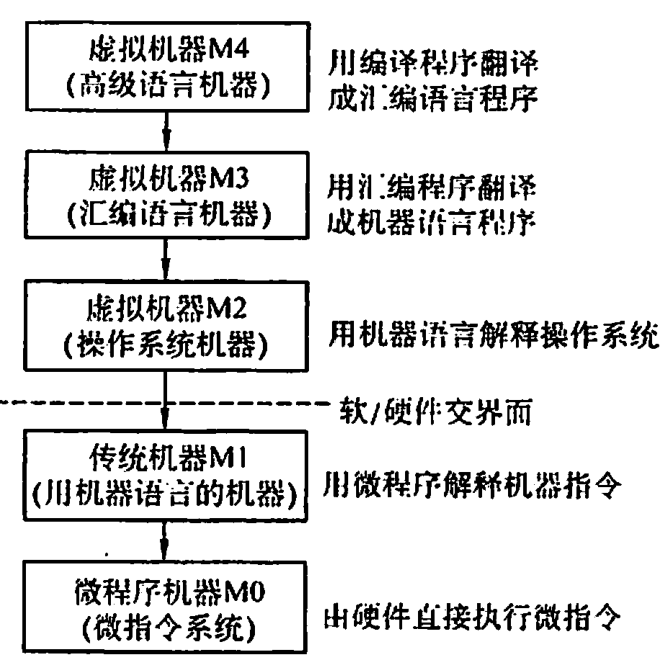
\includegraphics[width=0.4\textwidth]{./images/computer_system_layer.png}
  \caption{计算机系统的多级层次结构}
  \label{computer_system_layer}
\end{figure}

如图\ref{computer_system_layer}所示:
\begin{itemize}
  \item 第一级是微程序机器层,是实在的硬件层。
  \item 第二级是传统机器语言层,也是实在的硬件层。
  \item 第三级是操作系统层,这一层也成为混合层。
  \item 第四级是汇编语言层。
  \item 第五级是高级语言层。
\end{itemize}

软件和硬件的交界面就是ISA。

\subsubsection{计算机系统的工作原理}

\begin{enumerate}
  \item {\kaishu 从源程序到可执行文件}
  
  gcc编译流程:预处理-编译-汇编-链接
  \item {\kaishu 指令执行过程的描述}
  \begin{enumerate}
    \item 取指令:PC$\to$MAR$\to$M$\to$MDR$\to$IR
    \item 分析指令:OP(IR)$\to$CU
    \item 执行指令:Ad(IR)$\to$MAR$\to$M$\to$MDR$\to$ACC
  \end{enumerate}
  表示数据通路时括号可以省略,但运算时括号不能省略。如果题目中的括号没有省略,答题时也最好不要省略。
\end{enumerate}

\begin{problem}
  冯·诺依曼机的基本工作方式是 \uline{控制流驱动方式}。
\end{problem}

\begin{problem}
  下列(\ \ )不属于系统软件。
  \begin{enumerate}
    \item [A. ] 数据库系统
    \item [B. ] 操作系统
    \item [C. ] 编译程序
    \item [D. ] 以上三种都属于系统程序
  \end{enumerate}
\end{problem}

\begin{solution}
  A.本题易误选D。注意数据库系统=数据库+数据库管理系统+应用系统+数据库管理员,其中仅数据库管理系统是系统程序。
\end{solution}

\begin{problem}
  相联存储器 \uline{既可按地址寻址又可按内容寻址}。
\end{problem}

\begin{problem}
  【2009统考】冯·诺依曼计算机中指令和数据均以二进制形式存放在存储器中,CPU区分它们的依据是(\ \ )
  \begin{enumerate}
    \item [A. ] 指令操作码的译码结果
    \item [B. ] 指令和数据的寻址方式
    \item [C. ] 指令周期的不同阶段
    \item [D. ] 指令和数据所在的存储单元
  \end{enumerate}
\end{problem}

\begin{solution}
  C。通常取指阶段取出的是指令,执行阶段取出的是数据。
\end{solution}

\subsection{计算机的性能指标}

\subsubsection{计算机的主要性能指标}

\begin{enumerate}
  \item {\kaishu 字长},指计算机进行一次整数运算所能处理的二进制数据的位数。
  \item {\kaishu 数据通路带宽}
  \item {\kaishu 主存容量}。MAR的位数反映了存储单元的个数,MDR的位数反映了存储单元的字长。
  \item {\kaishu 运算速度}
  \begin{enumerate}
    \item 吞吐量,主要取决于主存的存储周期。
    \item 响应时间,通常包括CPU时间和等待时间。
    \item CPU时钟周期,是主频的倒数,是CPU中最小的时间单位。
    \item 主频。
    \item CPI:执行一条指令所需要的时钟周期数。一般是一个平均值。
    \item CPU执行时间
    \item MIPS:百万条指令每秒
    \item 浮点操作次数每秒系列单位:MFLOPS、GFLOPS、TFLOPS、PFLOPS、EFLOPS、ZFLOPS、EFLOPS
  \end{enumerate}
  注意:在描述存储容量、文件大小等时,K、M、G、T通常用2的幂次表示,而描述速率、频率等时,通常用10的幂次表示。
\end{enumerate}

\begin{problem}
  从用户观点看,评价计算机系统性能的综合参数是(\ \ )
  \begin{enumerate}
    \item [A. ] 指令系统
    \item [B. ] 吞吐率
    \item [C. ] 主存容量
    \item [D. ] 主频
  \end{enumerate}
\end{problem}

\begin{solution}
  B
\end{solution}

\section{数据的表示和运算}

\subsection{数制与编码}

\subsubsection{进位计数制及其相互转换}

计算机系统中所有信息都用二进制编码的原因:
\begin{itemize}
  \item 使用有两个稳定状态的物理器件就可以表示二进制数的每一位,成本低廉。
  \item 二进制的“0”和“1”恰好与逻辑值“真”和“假”相对应。
  \item 二进制的编码和运算规则都比较简单。
\end{itemize}

\begin{enumerate}
  \item {\kaishu 进位计数法}
  
  一个$r$进制数($K_n K_{n-1}\cdots K_0 K_{-1}\cdots K_{-m}$)的数值可表示为
  \begin{equation*}
    K_n r^n+K_{n-1}r^{n-1}+\cdots+K_0 r^0+K_{-1}r^{-1}+\cdots+K_{-m}r^{-m}=\sum_{i=n}^{-m}K_i r^i
  \end{equation*}
  式中,$r$是基数;$r^i$是第$i$位的位权(整数位最低规定为第0位);$K_i$的取值可以是$0,1,\cdots,r-1$共$r$个数码中的任意一个。
  \item {\kaishu 不同进制数之间的相互转换}
  \begin{enumerate}
    \item 二进制转八进制和十六进制
    
    二进制混合数(整数+小数)的整数部分,高位补0至对齐(转八进制则对齐到3位的整数倍,转十六进制则对齐到4位的整数倍);小数部分,低位补0至对齐,然后直接转换。

    八、十六进制互转时,可借助二进制作为中介。
    \item 任意进制数转为十进制数:各位数码和权值相乘然后加起来
    \item 十进制数转为任意进制数
    
    将十进制混合数拆成整数部分和小数部分,整数部分除基取余,小数部分乘基取整,最后再拼接起来。

    乘基取整:小数部分乘基取整,最先取得的整数为数的最高位,最后取得的整数为数的最低位,乘基为1.0或满足精度要求时结束。

    每个二进制小数都可以用十进制小数精确表示,但反之则不一定。
  \end{enumerate}
\end{enumerate}

\subsubsection{BCD码}

本节已从新大纲中删除,故略。

\subsubsection{定点数的编码表示}

\begin{enumerate}
  \item 机器数的定点表示
  \item 原码、反码、补码、移码
  \begin{enumerate}
    \item 原码表示法
    
    \begin{itemize}
      \item 若字长为$n+1$,则原码\textbf{小数}的表示范围为$-(1-2^{-n})\leq x\leq 1-2^{-n}$(关于原点对称)
      \item 若字长为$n+1$,则原码\textbf{整数}的表示范围为$-(2^{n}-1)\leq x\leq 2^{n}-1$(关于原点对称)
    \end{itemize}

    真值0的原码表示有两种,即+0和-0。
    \item 补码表示法
    
    小数补码比原码多表示一个-1,整数补码比原码多表示一个-2。

    变形补码:又称模4补码,双符号位的补码小数,符号位00表示正,11表示负。模4补码的符号位的存储仅仅需要\textbf{一位}而不是两位,因为任何一个正确的模4补码,符号位的两位都是相同的,如果不同表示发生了溢出。

    补码真值互转:整数直接按原码转换,负数则各位取反加1。

    另一种方法:从后往前找到第一个1,该1不变,前面所有位(含符号位)取反,符号去掉即可。
    \item 反码表示法
    \item 移码表示法
    
    移码就是在真值上加一个偏置值:
    \begin{equation*}
      [x]_{\text{移}}=2^n+x\ (-2^n\leq x< 2^n\text{,其中机器字长为}n+1)
    \end{equation*}
    移码有如下特点:
    \begin{itemize}
      \item 0的表示是唯一的。
      \item 同一个真值的补码和移码只差一个符号位。补码符号位取反,数值部分不变即得移码,反之亦然。
      \item 移码保持了数据的原有大小顺序,移码大真值就大,移码小真值就小。
    \end{itemize}
  \end{enumerate}
\end{enumerate}

\subsubsection{整数的表示}

\begin{enumerate}
  \item {\kaishu 无符号整数的表示}
  \item {\kaishu 带符号整数的表示}
\end{enumerate}

\begin{problem}
  对于相同位数(设为$N$位,不考虑符号位)的二进制补码小数和十进制小数,比值$\frac{\text{二进制小数能表示的数的个数}}{\text{十进制小数能表示的数的个数}}$为 \uline{$(0.2)^N$}
\end{problem}

\begin{solution}
  $N$位二进制小数可以表示的数的个数为$1+2^0+2^1+\cdots+2^{N-1}=2^N$,而十进制小数能表示的数的个数为$10^N$,二者的商为$(0.2)^N$。这也是计算机的运算中会出现误差的原因,它表明仅有$(0.2)^N$的概率的十进制数可以精确地用二进制表示。
\end{solution}

\subsection{运算方法和运算电路}

\subsubsection{基本运算部件}

408很少涉及本节内容。

加法器是ALU的核心部件。

\begin{enumerate}
  \item {\kaishu 一位全加器}
  \item {\kaishu 串行进位加法器}
  
  串行进位加法器的最长运算时间主要是由进位信号的传递时间决定的,加法器本身的求和时间只是次要因素。
  \item {\kaishu 并行进位加法器}
  \item {\kaishu 带标志加法器}
  \item {\kaishu 算数逻辑单元(ALU)}
\end{enumerate}

\subsubsection{定点数的移位运算}

\begin{enumerate}
  \item {\kaishu 算术移位}
  
  算术移位的对象是\textbf{有符号数}。

  算术移位不管怎么移,符号位永远是不变的,也即移位只作用于数值位。

  \begin{itemize}
    \item 正数无论码制,左右移都一律补0。
    \item 负数稍复杂:
    \begin{itemize}
      \item 原码:一律补0
      \item 反码:一律补1
      \item 补码:左移补0,右移补1
    \end{itemize}
  \end{itemize}

  \begin{table}[!ht]
    \centering
    \caption{不同机器数算术移位后的空位添补规则}
    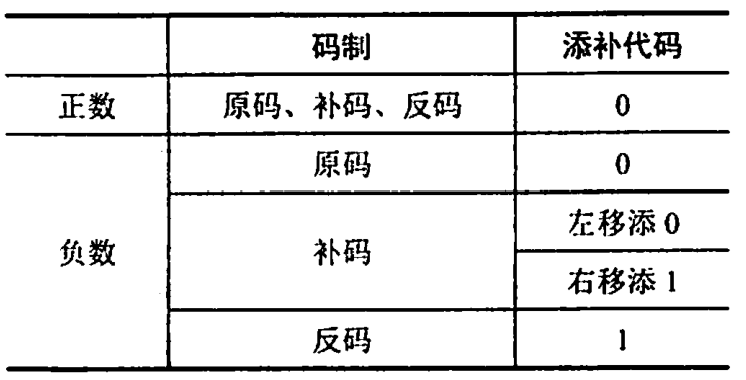
\includegraphics[width=0.6\textwidth]{./images/shift_rule.png}
  \end{table}
  \item {\kaishu 逻辑移位}
  
  逻辑移位将移位对象视为\textbf{无符号数}。无论码制、左右移,一律补0。
  \item {\kaishu 循环移位}
  
  又分带进位标志CF的循环移位和不带进位标志的循环移位。

  带CF的循环移位是将移出的位送入标志位CF,并将CF的值送入腾出的位。

  即使是不带CF的循环移位,实际上CF的值也是会变的,但CF只是单纯输入,不再输出。输入的值是移出的位。

  循环移位操作常用于交换寄存器的高低字节。
\end{enumerate}

\subsubsection{定点数的加减运算}

\begin{enumerate}
  \item {\kaishu 补码的加减法运算}
  \item {\kaishu 补码加减运算电路}
  
  这里有一个各标志位的含义,可能有用。待补。
  \item {\kaishu 溢出判别方法}
  
  仅当两个符号相同的数相加或者两个符号相异的数相减才有可能产生溢出。判断溢出的方法有三种:
  \begin{itemize}
    \item 采用一位符号位:无论加减,只要参加操作的两个数符号相同,结果又与源操作数符号不同,就表示溢出。
    \item 采用双符号位:运算结果的两个符号位相同,表示未溢出;若不同则表示溢出。
    \begin{itemize}
      \item 00:表示结果为正,无溢出。
      \item 01:表示结果正溢出。
      \item 10:表示结果负溢出。
    \end{itemize}
    \item 采用一位符号位根据数据位的进位情况判断溢出
    
    当最高符号位的进位和数值位的进位不同时,说明发生溢出。
  \end{itemize}
\end{enumerate}

\subsubsection{定点数的乘除运算}

待补

\subsubsection{C语言中的整数类型及类型转换}

本节为408常考内容。

当大字长变量向小字长变量强制类型转换时,多余的高位直接截掉,低位直接赋值,而不是进行类似循环溢出的操作。

短字长向长字长转换时,不仅要使相应的位值相等,还要对高位进行扩展:
\begin{itemize}
  \item 如果原数字是无符号整数,则进行零扩展
  \item 如果原数字带符号,则进行符号扩展。
\end{itemize}

char类型为8位无符号整数,转为int时高位补0即可。

\subsubsection{数据的存储和排列}

\begin{enumerate}
  \item {\kaishu 数据的“大端方式”和“小端方式”存储}
  \begin{itemize}
    \item 大端:低字节放高地址
    \item 小端:低字节放低地址
  \end{itemize}
  \item {\kaishu 数据按“边界对齐”方式存储}
  
  \textbf{注意}:题目涉及\textbf{结构体}的,一定要留意对齐方式(一般都是边界对齐的)!
\end{enumerate}

\subsection{浮点数的表示与运算}

\subsubsection{浮点数的表示}

\begin{enumerate}
  \item {\kaishu 浮点数的表示格式}
  
  通常,浮点数可表示为
  \begin{equation*}
    N=(-1)^S\times M\times R^E
  \end{equation*}
  其中:
  \begin{itemize}
    \item $S$决定浮点数的符号,可取0或1。
    \item $M$是尾数,是一个二进制定点小数,通常用原码表示。
    \item $E$是阶码,是一个二进制定点整数,通常用移码表示。
    \item $R$是隐含的基数,可取2、4、16等。
  \end{itemize}
  \item {\kaishu 浮点数的表示范围}
  
  \begin{itemize}
    \item 数据产生上溢(正上溢、负上溢)时,计算机必须停机处理溢出。
    \item 数据产生下溢(正下溢、负下溢)时,计算机将其当作机器零处理。
  \end{itemize}
  \item {\kaishu 浮点数的规格化}
  
  \begin{itemize}
    \item 左规:尾数的最高位不是有效位,即尾数为$0.0\cdots$时,进行左规,尾数每左移一次,阶码减一(仅基数为2时)。
    \item 右规:尾数的有效位进到小数点前面时,进行右规,尾数右移一位,阶码加一(仅基数为2时)。
  \end{itemize}

  基数不同,浮点数的规格化形式也不同。基数为2时,原码规格化数的尾数最高位一定是1;基数为4时,原码规格化形式的尾数最高两位不全为0。
  \item {\kaishu IEEE 754标准}
  
  IEEE 754规定:浮点数的基数隐含为2,尾数采用隐藏位策略的原码表示,阶码用移码表示。
  \begin{table}
    \centering
    \caption{IEEE 754浮点数的格式}
    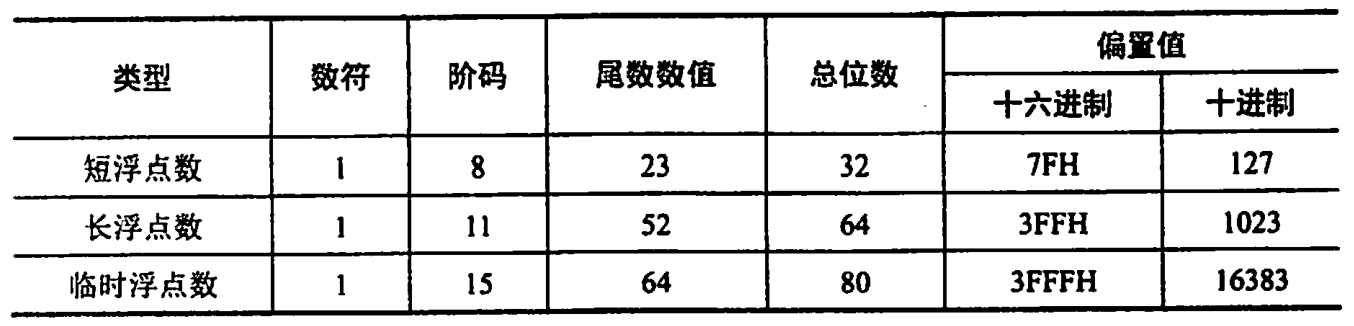
\includegraphics[width=0.7\textwidth]{./images/ieee754.png}
  \end{table}
  对于短浮点数,偏置值为127;对于长浮点数,偏置值为1023。存储阶码之前,要先把真值加上偏置值;反之在解析真值时,需要将阶码减去偏置值。

  规格化的二进制浮点数,数值最高位总是1,因此此位省略,尾数实际上能多表示一位有效位。
  \item {\kaishu 定点、浮点表示的区别}
\end{enumerate}

\subsubsection{浮点数的加减运算}

分为以下几步:
\begin{enumerate}
  \item {\kaishu 对阶}
  
  原则是小阶向大阶对齐,即将阶码数小的浮点数的阶码逐位增加1,同时尾数逐位右移,直到两个数阶码相等为止。
  \item {\kaishu 尾数求和}
  \item {\kaishu 规格化}
  
  尾数求和的结果不一定是规格化的,因此需要规格化。
  \item {\kaishu 舍入}
  
  为保证精度,一般将右移移出的位保留下来,在最后得出结果时舍入成IEEE 754格式。
  \begin{itemize}
    \item 0舍1入法:类似四舍五入。若保留下来的最高位为1,则在尾数的末位加1,否则就舍去。
    \item 恒置1法:无脑将右移后的尾数末位置为1。
    \item 截断法:直接截断,最简单。
  \end{itemize}
  \item {\kaishu 溢出判断}
\end{enumerate}

\section{存储系统}

\subsection{存储器概述}

\subsubsection{存储器的分类}

\begin{enumerate}
  \item {\kaishu 按在计算机中的作用(层次)分类}
  \begin{itemize}
    \item 主存储器
    \item 辅助存储器
    \item 高速缓冲存储器(Cache)
  \end{itemize}
  \item {\kaishu 按存储介质分类}
  \begin{itemize}
    \item 磁表面存储器(磁盘、磁带)
    \item 磁芯存储器
    \item 半导体存储器
    \begin{itemize}
      \item MOS型存储器
      \item 双极型存储器
    \end{itemize}
    \item 光存储器(光盘)
  \end{itemize}
  \item {\kaishu 按存取方式分类}
  \begin{itemize}
    \item 随机存储器(RAM):又分静态RAM和动态RAM
    \item 只读存储器(ROM):可与RAM共同作为主存的一部分,统一构成主存的地址域。\textbf{同样支持随机访问}。
    \item 串行访问存储器。包括:
    \begin{itemize}
      \item 顺序存取存储器(如磁带)
      \item 直接存取存储器(如磁盘、光盘)
    \end{itemize}
  \end{itemize}
  \item {\kaishu 按信息的可保存性分类}
  \begin{itemize}
    \item 易失性存储器,如RAM
    \item 非易失性存储器,如ROM、磁表面存储器和光存储器。
  \end{itemize}
\end{enumerate}

\subsubsection{存储器的性能指标}

三大性能指标:
\begin{enumerate}
  \item 存储容量。=存储字数$\times$字长
  \item 单位成本。
  \item 存储速度。
  \begin{itemize}
    \item 存取时间:启动一次存储器操作到完成该操作所经历的时间。
    \item 存取周期:又称读写周期或访问周期,是指存储器进行一次完整的读写操作所需的全部时间,即连续两次独立访问存储器操作之间所需的最小时间间隔。
    \item 主存带宽:表示每秒从主存进出信息的最大数量。
  \end{itemize}
  存取周期通常大于存取时间。因为存储器在读写操作之后往往需要一段恢复内部状态的复原时间。即
  \begin{equation*}
    \text{存取周期}=\text{存取时间}+\text{恢复时间}
  \end{equation*}
\end{enumerate}

\subsubsection{多级层次的存储系统}

存储系统层次结构主要体现在Cache-主存层和主存-辅存层。

\begin{itemize}
  \item 主存和Cache之间的数据调动由硬件自动完成,对所有程序员都是透明的。
  \item 主存和辅存之间的数据调动由硬件和操作系统共同完成,对应用程序员是透明的。
\end{itemize}

\subsection{主存储器}

\subsubsection{SRAM芯片和DRAM芯片}

DRAM的常见刷新方式:
\begin{itemize}
  \item 集中刷新:在一个规定的\textbf{刷新周期}内,对所有行进行刷新。这段时间 RAM 无法读写,也即存在死区。
  \item 分散刷新:将刷新分散到每个存取周期中进行。无死区,但存取周期变长。
  \item 异步刷新:二者的结合。顺序刷新各行。也有死区,但是死区时间变短。
\end{itemize}

DRAM的刷新单位是行,刷新时不需要选片,因为所有芯片同时被刷新。

SRAM和DRAM的比较见表\ref{sram_and_dram}。

\begin{table}
  \centering
  \caption{SRAM和DRAM各自的特点}
  \label{sram_and_dram}
  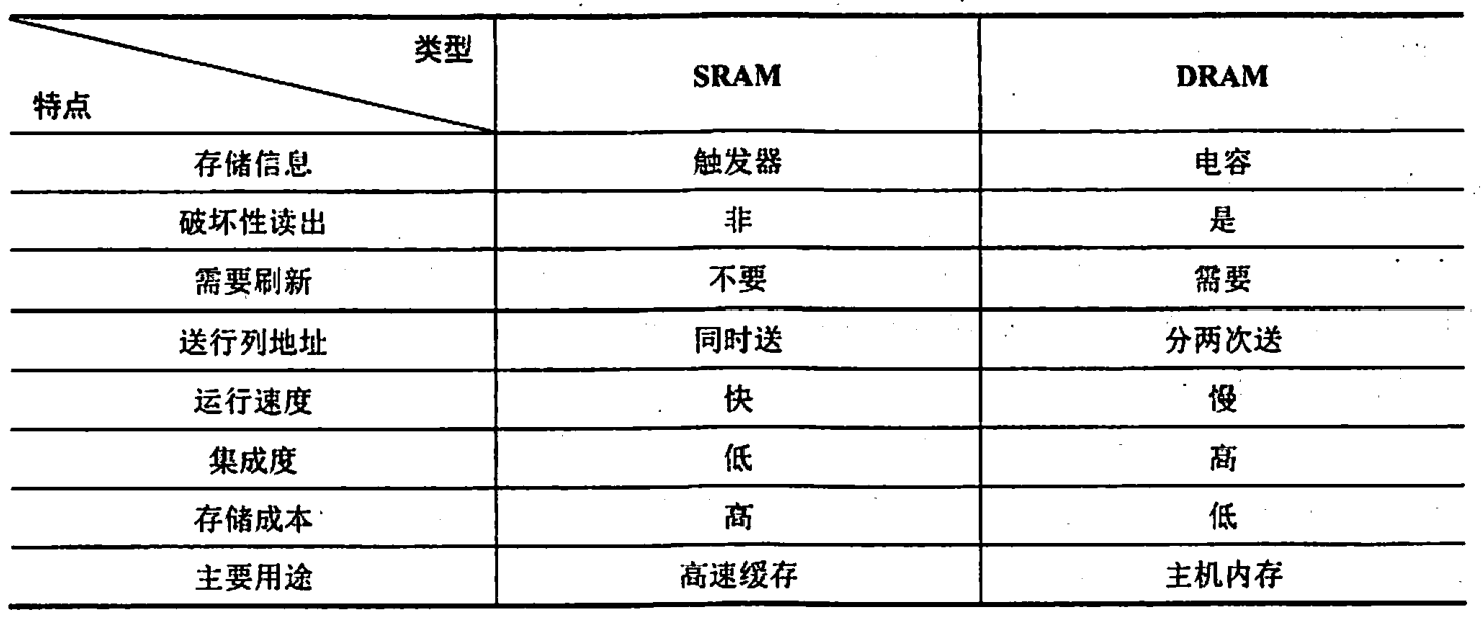
\includegraphics[width=0.7\textwidth]{./images/sram_and_dram.png}
\end{table}

\subsubsection{只读存储器ROM}

ROM包括MROM、PROM、EPROM、EEPROM、Flash等。

\subsubsection{主存储器的基本组成}

本节易考“芯片最少需要多少引脚”的问题。

对于SRAM,地址线的条数是存储单元数量的对数(行列信号同时传输),而数据线的条数就是一个存储单元的长度,此外还要附加若干条片选线(根据芯片数量确定,一片芯片时片选线为一位宽)和读写控制线。读写控制线一般为2条(WE、RD)。

对于DRAM,一般采用地址复用技术。地址线的数量应当减半,同时片选线数量应该加倍,因为分出了行通选线和列通选线(先行后列)。其他和SRAM一致。

\begin{problem}
  某一SRAM芯片,其容量为$1024\times 8$位,除电源和接地端外,该芯片的引脚的最小数目为 \uline{21}。
\end{problem}

\begin{solution}
  地址线10条,数据线8条,片选线1条,读写控制线2条,共21条。
\end{solution}

\begin{problem}
  某一DRAM芯片,采用地址复用技术,容量为$1024\times 8$位,除电源线和接地端外,该芯片的引脚数最少是 \uline{17}。
\end{problem}

\begin{solution}
  地址线5($10\div 2$)条,数据线8条,片选线2条(行通选+列通选),控制线2条,共17条。
\end{solution}

\subsubsection{多模块存储器}

\begin{enumerate}
  \item {\kaishu 单体多字存储器}
  
  一次并行读出$m$个字,要求指令和数据必须连续存放。
  \item {\kaishu 多体并行存储器}
  \begin{itemize}
    \item 高位交叉编址(顺序方式)
    
    不能提高存储器的吞吐率。
    \item 低位交叉编址(408常用的名字是“交叉方式”)
    
    假设模块存取一个字的存取周期为$T$,总线传送周期为$r$,为实现流水线方式存取(某个模块被再次访问时已经准备好),存储器交叉模块数应大于等于
    \begin{equation*}
      m=\frac{T}{r}
    \end{equation*}
    其中$m$称为交叉存取度。每隔$r$时间延迟后启动下一个模块。这样,连续存取$m$个字所需的时间为
    \begin{equation*}
      t_1=T+(m-1)r
    \end{equation*}
    而顺序方式连续读取$m$个字所需的时间为$t_2=mT$。
  \end{itemize}
\end{enumerate}

\subsection{主存储器与CPU的连接}

\subsubsection{连接原理}

略

\subsubsection{主存容量的扩展}

\begin{enumerate}
  \item {\kaishu 位扩展法}
  
  各芯片连接地址线的方式相同,但连接数据线的方式不同,在某一时刻选中所有的芯片,所以片选信号要连接到所有的芯片。
  \item {\kaishu 字扩展法}
  
  各芯片连接地址线的方式相同,连接数据线的方式也相同,在某一时刻只需选中部分芯片,所以将片选信号直接连接到相应的芯片,或者通过译码器连接。
  \item {\kaishu 字位同时扩展法}
\end{enumerate}

注意:MAR的位数应该和CPU支持的内存大小保持一致,而不是和系统安装的内存大小保持一致。

\subsubsection{存储芯片的地址分配和片选}

\begin{enumerate}
  \item {\kaishu 线选法}
  \item {\kaishu 译码片选法}
\end{enumerate}

\begin{problem}
  【2018统考】假定DRAM芯片中存储阵列的行数为$r$、列数为$c$,对于一个2K$\times$1位的DRAM芯片,为保证其地址引脚数最少,并尽量减小刷新开销,则$r$、$c$的取值分别是(\ \ )
  \begin{enumerate}
    \item [A. ] 2048, 1
    \item [B. ] 64, 32
    \item [C. ] 32, 64
    \item [D. ] 1, 2048
  \end{enumerate}
\end{problem}

\begin{solution}
  C。为什么不选D?注意到DRAM采用行列地址线复用技术,这要求地址线需要和行数及列数中较大的那个保持一致。也就是说,行数和列数不能差得太多。
\end{solution}

\subsection{外部存储器}

磁盘的平均存储时间=寻道时间+旋转延迟时间+传输时间。其中寻道时间和旋转延迟时间通常取平均值。

磁盘地址=驱动器号+柱面号+盘面号+扇区号。

磁盘的读写操作是串行的,不可能在同一时刻既读又写。

\subsection{高速缓冲存储器}

\subsubsection{程序访问的局部性原理}

略

\subsubsection{Cache的基本工作原理}

\begin{itemize}
  \item CPU和Cache之间的数据交换以\textbf{字}为单位
  \item Cache与主存之间的数据交换则以\textbf{Cache块}为单位
\end{itemize}

设某个程序执行期间,Cache的总命中次数为$N_c$,访问主存的总次数为$N_m$,则命中率为
\begin{equation*}
  H=\frac{N_c}{N_c+N_m}
\end{equation*}

设$t_c$为命中时的Cache访问时间,$t_m$为未命中时的访问时间,$1-H$表示未命中率,则Cache-主存系统的平均访问时间$T_a$为
\begin{equation*}
  T_a=Ht_c+(1-H)t_m
\end{equation*}

\subsubsection{Cache和主存的映射方式}

\begin{itemize}
  \item 为了说明当前Cache块对应主存中的哪一块,需要为每个Cache块添加一个\textbf{标记(tag)}。
  \item 为了说明Cache行中的信息是否有效,需要为每个Cache行添加一个\textbf{有效位(valid bit)}。
\end{itemize}

地址映射有如下三种方法:
\begin{enumerate}
  \item {\kaishu 直接映射}
  
  \begin{equation*}
    \text{Cache行号}=\text{主存块号}\ \  mod\ \  \text{Cache总行数}
  \end{equation*}
  假设Cache有$2^c$行,主存有$2^m$块。上式表明,主存块号的低$c$位正好是它要装入的Cache行号。给每个Cache行设置一个长为$t=m-c$的标记(tag),当主存某块调入Cache后,就将其块号的高$t$位设置在对应Cache行的标记中。
  \item {\kaishu 全相联映射}
  
  \begin{itemize}
    \item 优点:灵活,Cache块的冲突概率低,空间利用率高,命中率也高;
    \item 缺点:标记的比较速度慢,实现成本高,通常需要采用昂贵的\textbf{按内容寻址}的相联存储器进行地址映射。
  \end{itemize}
  \item {\kaishu 组相联映射}
  
  将Cache分成若干个大小相等的组,组间采用直接映射,组内采用全相联映射。这是对上面两种方式的折中。

  组相联的成本接近直接映射,性能接近全相联映射。
\end{enumerate}

\subsubsection{Cache中主存块的替换算法}

可结合《操作系统》复习。

常见算法:
\begin{itemize}
  \item 随机算法
  \item 先进先出算法(FIFO)
  \item 近期最少使用算法(LRU)
  \item 最不经常使用算法
\end{itemize}

\subsubsection{Cache写策略}

\begin{itemize}
  \item 写命中
  \begin{itemize}
    \item 写直达法(write-through):写命中时,数据同时写入Cache和主存。
    \begin{itemize}
      \item 优点:简单,能随时保持主存数据的正确性。
      \item 缺点:增加了访存次数,降低了Cache的效率。
    \end{itemize}
    \item 写回法(write-back):写命中时,仅仅把数据写入Cache,而不立即写入主存。仅当此块被换出时才写回主存。
    \begin{itemize}
      \item 优点:减少了访存次数。
      \item 缺点:存在不一致的隐患。需要为每个Cache行设置一个脏位。
    \end{itemize}
  \end{itemize}
  \item 写不命中
  \begin{itemize}
    \item 写分配法(write-allocate):加载主存中的块到Cache中,然后更新这个Cache块。
    \item 写不分配法(not-write-through):只写入主存,不动Cache。
  \end{itemize}
  写不分配经常和写直达法搭配,写分配经常和写回法搭配。
\end{itemize}

\subsection{虚拟存储器}

\subsubsection{虚拟存储器的基本概念}

虚拟存储器将主存或辅存的地址空间统一编址,形成一个庞大的地址空间。

由于访问外存速度很慢,代价太高,相比Cache系统,虚拟存储器的命中率至关重要,因此虚拟存储器使用\textbf{全相联映射},主存中的任意一个虚页面都可以存储外存中的任意虚页面。

\subsubsection{页式虚拟存储器}

可参考《操作系统》,下同。

\subsubsection{段式虚拟存储器}

\subsubsection{段页式虚拟存储器}

\subsubsection{虚拟存储器和Cache的比较}

\begin{enumerate}
  \item {\kaishu 相同之处}
  
  \begin{itemize}
    \item 都是为了提高系统性能。
    \item 都把数据分成小块,并作为基本的传递单位。虚拟存储器的块更大。
    \item 都有地址的映射、替换、更新策略等问题。
    \item 都利用了程序的局部性原理,将活跃数据放在相对高速的部件中。
  \end{itemize}
  \item {\kaishu 不同之处}
  
  \begin{itemize}
    \item Cache主要解决系统速度问题,虚拟存储器主要解决主存容量问题。
    \item Cache全部由硬件实现,对所有程序员透明;虚拟存储器由OS和硬件共同实现,对应用程序员不透明但对系统程序员透明。
    \item 虚拟存储器不命中对性能的影响更大。
    \item CPU和主存有直接通路,但和外存没有直接通路。这意味着Cache不命中时CPU可直接到主存调取数据,但虚拟内存不命中时CPU必须等待数据调入主存后再访问。
  \end{itemize}
\end{enumerate}

\begin{problem}
  Cache行的大小和命中率之间有什么关系?
\end{problem}

\begin{solution}
  \begin{itemize}
    \item 行的长度较大,可以充分利用空间局部性,使一个更大的局部空间被整体调入Cache,从而增加命中的机会。
    \item 行的长度太大时,会导致:
    \begin{itemize}
      \item 失效损失变大。未命中时需要消耗更多时间从主存读取。
      \item Cache的项数变少,命中的可能性变小。
    \end{itemize}
  \end{itemize}
\end{solution}

\section{指令系统}

\subsection{指令系统}

指令系统是ISA的最核心部分。

\subsubsection{指令的基本格式}

指令=操作码+地址码。

指令的长度和机器字长没有固定的关系,可能大于也可能小于。指令字长一般是字节的整数倍。

根据指令的地址码数量不同,可分为:
\begin{enumerate}
  \item {\kaishu 零地址指令}
  
  仅有一个操作码。有两种情况:
  \begin{itemize}
    \item 不需要操作数的指令。如空操作、停机、关中断等。
    \item 运算类指令,但运算类的零地址指令只存在于堆栈计算机。两个操作数一般来自栈顶和次栈顶。
  \end{itemize}
  \item {\kaishu 一地址指令}
  
  同样有两种情况:
  \begin{itemize}
    \item 只需要一个操作数,如加一、减一、求反、求补等。
    \item 需要两个操作数,另一个操作数是隐含的,来自累加器ACC。
  \end{itemize}
  \item {\kaishu 二地址指令}
  \item {\kaishu 三地址指令}
  
  除了两个操作数之外,还提供结果地址,运算结果将送入结果地址。
  \item {\kaishu 四地址指令}
  
  除了两个操作数、结果地址之外,还提供下一条指令的地址。
\end{enumerate}

\textbf{注意}:指令的地址数$\neq$操作数的数量。有些指令会隐含操作数,此时地址数要小于操作数的数量。

\subsubsection{定长操作码指令格式}

多用于32位或更多字长的计算机。

\subsubsection{扩展操作码指令格式}

这种格式的目的是保持指令字长不变,同时增加操作码的数量。

注意事项:
\begin{itemize}
  \item 不允许短码是长码的前缀。
  \item 各个指令的操作码一定不能重复。
\end{itemize}

一般对使用频率较高的指令分配较短的操作码,反之分配较长的操作码,以减少指令译码和分析的时间。

\subsubsection{指令的操作类型}

\begin{enumerate}
  \item {\kaishu 数据传送}
  \item {\kaishu 算术和逻辑运算}
  \item {\kaishu 移位操作}
  \item {\kaishu 转移操作}
  \item {\kaishu 输入输出操作}
\end{enumerate}

\begin{problem}
  【2022统考】设计某指令系统时,假设采用16位定长指令字格式,操作码使用扩展编码方式,地址码为6位,包含零地址,一地址和二地址3种格式的指令。若二地址指令有12条,一地址指令有254条,则零地址指令的条数最多为(\ \ )
  \begin{enumerate}
    \item [A. ] 0
    \item [B. ] 2
    \item [C. ] 64
    \item [D. ] 128
  \end{enumerate}
\end{problem}

\begin{solution}
  D。地址码为6位,一条二地址指令会占用$2^6$条一地址指令的空间,一条一地址指令会占用$2^6$条零地址指令的空间,如果全都是零地址指令,则最多有$2^{16}$条,减去一地址指令和二地址指令所占用的零地址指令空间,即
  \begin{equation*}
    2^{16}-254\times 2^6-12\times 2^6\times 2^6=128
  \end{equation*}
\end{solution}

\subsection{指令的寻址方式}

寻址方式=指令寻址+数据寻址

\subsubsection{指令寻址和数据寻址}

\begin{enumerate}
  \item {\kaishu 指令寻址},又包括
  \begin{itemize}
    \item 顺序寻址
    \item 跳跃寻址
  \end{itemize}
  \item {\kaishu 数据寻址}
  
  方式众多。一般在指令字中设置一个字段,指明属于哪种寻址方式。
\end{enumerate}

\subsubsection{常见的数据寻址方式}

细节待补

\begin{enumerate}
  \item {\kaishu 隐含寻址}
  \item {\kaishu 立即(数)寻址}
  \item {\kaishu 直接寻址}
  \item {\kaishu 间接寻址}
  \item {\kaishu 寄存器寻址}
  \item {\kaishu 寄存器间接寻址}
  \item {\kaishu 相对寻址}
  \item {\kaishu 基址寻址}
  \item {\kaishu 变址寻址}
  \item {\kaishu 堆栈寻址}
\end{enumerate}

\subsection{程序的机器级表示}

本节是2022大纲新增考点。

AT\&T格式汇编和Intel格式汇编的比较:
\begin{itemize}
  \item AT\&T只能用小写字母,Intel则大小写均可。
  \item AT\&T的目的操作数在后,Intel的目的操作数在前。
  \item AT\&T格式中,寄存器前面要加\%,立即数前面要加\$,Intel格式则无需前缀。
  \item 内存寻址方面,AT\&T格式使用小括号,Intel格式使用中括号。
  \item 处理复杂寻址方式时,AT\&T的"\verb|disp(base, index, scale)|"等价于Intel的“\verb|[base + index * scale + disp]|”。
  \item 指定数据长度方面,AT\&t在操作码的后面紧跟一个字符,如“b”“w”等;Intel则使用“\verb|byte ptr|”“\verb|word ptr|”等。
\end{itemize}

常用指令:待补

\subsubsection{过程调用的机器级表示}

待补

\subsubsection{选择语句的机器级表示}

条件码:
\begin{itemize}
  \item {\bf CF}:进(借)位标志。最近的\textbf{无符号数}加减运算后的进借位情况。有为1,无为0。
  \item {\bf ZF}:零标志。
  \item {\bf SF}:符号标志。最近的\textbf{带符号数}运算结果的符号。负为1。
  \item {\bf OF}:溢出标志。最近的\textbf{带符号数}运算是否产生溢出。溢出为1。
\end{itemize}

其余内容待补

\subsubsection{循环语句的机器级表示}

待补

\subsection{CISC和RISC的基本概念}

\subsubsection{复杂指令系统计算机 CISC}

主要特点:
\begin{itemize}
  \item 指令系统庞大复杂,指令数量多。
  \item 指令长度不固定,格式多样,寻址方式多样。
  \item 许多指令都可以访存。
  \item 各种指令使用频率相差很大。
  \item 各种指令执行时间相差很大。多数指令需要多个时钟周期完成。
  \item 控制器多采用微程序控制。逻辑过于复杂以至于无法用硬连线控制。
  \item 难以进行编译优化。
\end{itemize}

\subsubsection{精简指令系统计算机 RISC}

主要特点:
\begin{itemize}
  \item 指令数量少,每条指令都很简单,通过指令的组合来实现复杂的功能。
  \item 指令长度固定,格式种类少,寻址方式种类少。
  \item 仅用load/store指令访存。
  \item CPU往往有较多的通用寄存器。
  \item \textbf{一定}采用流水线技术,大部分指令在一个时钟周期内完成。
  \item 控制器多采用硬连线控制。
  \item 特别重视编译优化。
\end{itemize}

\subsubsection{CISC和RISC的比较}

CISC对老机器的兼容性比RISC好。

\section{中央处理器}

\subsection{CPU的功能和基本结构}

\subsubsection{CPU的功能}

\begin{enumerate}
  \item {\kaishu 指令控制}
  \item {\kaishu 操作控制}
  \item {\kaishu 时间控制}
  \item {\kaishu 数据加工}
  \item {\kaishu 中断处理}
\end{enumerate}

\subsubsection{CPU的基本结构}

CPU=运算器+控制器

\begin{enumerate}
  \item {\kaishu 运算器}
  \begin{itemize}
    \item 算术逻辑单元ALU
    \item 暂存寄存器
    \item 累加寄存器ACC
    \item 通用寄存器组
    \item 程序状态字寄存器
    \item 移位器
    \item 计数器
  \end{itemize}
  \item {\kaishu 控制器}
  \begin{itemize}
    \item 程序计数器PC
    \item 指令寄存器IR
    \item 指令译码器
    \item 存储器地址寄存器MAR
    \item 存储器数据寄存器MDR
    \item 时序系统,都由统一时钟分频得到。
    \item 微操作信号发生器
  \end{itemize}
  控制器有硬布线控制器和微程序控制器两种。
\end{enumerate}

CPU内部的寄存器可以分成两类:
\begin{itemize}
  \item 用户可见的寄存器,可以编程,如通用寄存器组、程序状态字寄存器。
  \item 用户不可见的寄存器,对用户透明,不可编程,如MAR、MDR、IR。
\end{itemize}

所谓的$n$位CPU中,$n$指的是\textbf{数据总线线数}。

\begin{problem}
  在一条无条件跳转指令的指令周期内,PC的值被修改(\ \ )次。
  \begin{enumerate}
    \item [A. ] 1
    \item [B. ] 2
    \item [C. ] 3
    \item [D. ] 无法确定
  \end{enumerate}
\end{problem}

\begin{solution}
  B。取值周期结束后,PC值自动加1;执行周期中,PC值修改为要跳转到的地址,因此被修改两次。
\end{solution}

\subsection{指令执行过程}

\subsubsection{指令周期}
\label{instruction_cycle}

CPU从主存中\textbf{取出并执行}一条指令的时间称为\textbf{指令周期}。

指令周期通常用若干机器周期来表示,一个机器周期又包含若干个时钟周期(又叫节拍)。时钟周期是CPU操作的最基本单位。

访问一次存储器的时间是固定的,因此通常用存取周期作为机器周期。机器周期是人为规定的。

每个指令周期内的机器周期数可以不等,每个机器周期内的时钟周期也可以不等。

一个完整的指令周期依次是:
\begin{itemize}
  \item 取指 FE
  \item 间址 IND
  \item 执行 EX
  \item 中断 INT
\end{itemize}

注意:中断周期中的进栈操作是将SP减1,这和传统意义上的进栈操作相反,原因是计算机中的堆栈向低地址增加。

\subsubsection{指令周期的数据流}

\begin{enumerate}
  \item {\kaishu 取指周期}
  
  取指令的同时,PC+1。
  \item {\kaishu 间址周期}
  \item {\kaishu 执行周期}
  \item {\kaishu 中断周期}
  
  进栈操作是先修改栈顶指针,再存入数据。
\end{enumerate}

\subsubsection{指令执行方案}

\begin{enumerate}
  \item {\kaishu 单指令周期}:对所有指令都用相同的时间执行,指令是串行执行的。每条指令都用一个时钟周期执行完成,因此时钟周期取决于执行时间最长的指令。
  \item {\kaishu 多指令周期}:对不同指令使用不同数量的时钟周期执行,但指令仍然是串行执行的。
  \item {\kaishu 流水线方案}:略
\end{enumerate}

\begin{problem}
  采用DMA方式传递数据时,每传送一个数据就要占用 \uline{存取周期}。
\end{problem}

\textbf{在指令长度相同的情况下},所有指令的取指操作是相同的。

指令字长一般都取存储字长的整数倍,若指令字长等于存储字长的两倍,则需要两次访存,取指周期等于机器周期的两倍。若指令字长等于存储字长,则取指周期等于机器周期。

\subsection{数据通路的功能和基本结构}

\subsubsection{数据通路的功能}

数据在功能部件之间传送的路径称为数据通路。

\subsubsection{数据通路的基本结构}

有以下几种:
\begin{enumerate}
  \item {\kaishu CPU内部单总线方式},将所有寄存器的输入、输出端都连接到一条公共通路上,结构简单,但有很多冲突。
  \item {\kaishu CPU内部多总线方式}。
  \item {\kaishu 专用数据通路方式}。不用共享总线,而是根据数据通路设计特定的连线,性能很好,但硬件量很大。
\end{enumerate}

单总线结构中,ALU的两个输入端不能都连接到总线,而是一端连总线,另一端通过一个寄存器间接地连接总线。输出端也必须通过一个寄存器间接连接总线。

\begin{problem}
  【2016统考】单周期处理器中所有指令的指令周期为一个时钟周期。下列关于单周期处理器的叙述中,错误的是(\ \ )
  \begin{enumerate}
    \item [A. ] 可以采用单总线结构数据通路
    \item [B. ] 处理器时钟频率较低
    \item [C. ] 在指令执行过程中控制信号不变
    \item [D. ] 每条指令的CPI为1
  \end{enumerate}
\end{problem}

\begin{solution}
  A。单总线结构每个时钟周期只能完成一个操作,但一条指令无疑需要多个操作,因此不能用于单周期处理器。
\end{solution}

\subsection{控制器的功能和工作原理}

\subsubsection{控制器的结构和功能}

控制器的功能有:
\begin{enumerate}
  \item 从主存中取出一条指令,并指出下一条指令在主存中的位置。
  \item 对指令进行译码或测试,产生相应的操作控制信号,以便启动规定的动作。
  \item 指挥并控制CPU、主存、输入和输出设备之间的数据流动方向。
\end{enumerate}

\subsubsection{硬布线控制器}

又称组合逻辑控制器。

\begin{figure}
  \centering
  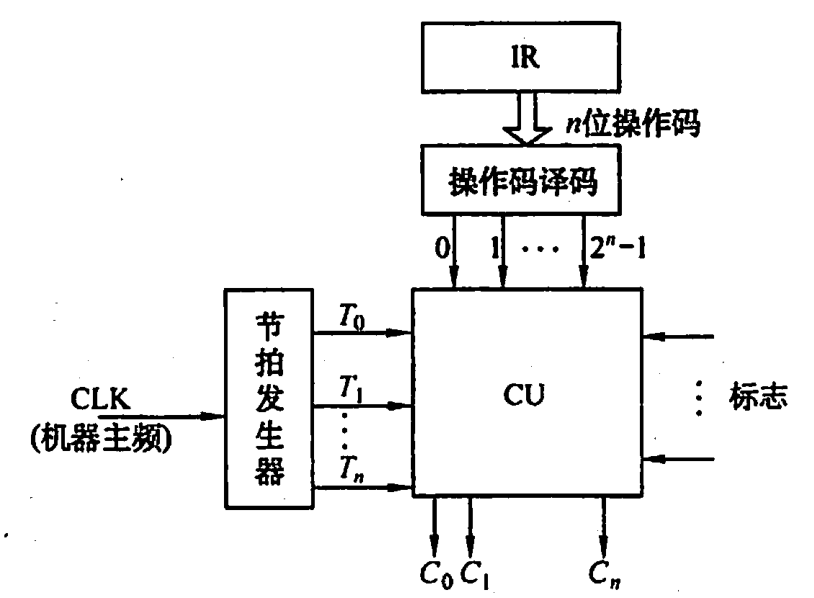
\includegraphics[width=0.5\textwidth]{./images/cu_with_id_and_clock_input.png}
  \caption{带指令译码器和节拍输入的控制单元图}
\end{figure}

CU的输入来自操作码译码电路ID、节拍发生器、状态标志,以及其他来自控制总线的中断请求、DMA请求等,并将输出发送到控制总线。

指令周期、机器周期、时钟周期:回顾\ref{instruction_cycle}节。

每个时钟周期(节拍)内,机器可以完成一个或几个需要同时执行的操作。

CPU的控制方式:
\begin{itemize}
  \item 同步控制方式,所有的控制信号同步到一个统一的系统时钟。控制电路简单,但运行速度慢。
  \item 异步控制方式:完全不同步,各个部件按照自身的速度工作,通过应答方式联络。速度快,但控制电路复杂。
  \item 联合控制方式:二者的折中。对于不同的微操作采用大部分同步、小部分异步的方法。
\end{itemize}

\subsubsection{微程序控制器}

将每条机器指令编写成一个\textbf{微程序},每个微程序包含若干\textbf{微指令},每条伪指令对应一个或几个\textbf{微操作命令}。

存放微指令的控制存储器的单元地址称为\textbf{微地址}。一条微指令通常包含:
\begin{itemize}
  \item {\bf 操作控制字段},又称微操作码字段,用于产生某一步操作所需的各种操作控制信号。
  \item {\bf 顺序控制字段},又称微地址码字段,用于控制产生下一条微指令的地址。
\end{itemize}

\textbf{微周期}是指执行一条微指令需要的时间,一般就是一个时钟周期。

存在类似主存的\textbf{控制存储器}(CM),用于存放微程序,集成在CPU内部,\textbf{用ROM实现}。

区分以下寄存器:
\begin{itemize}
  \item 地址寄存器MAR
  \item 微地址寄存器CMAR,用于存放待读/写的微指令的地址
  \item 指令寄存器IR
  \item 微指令寄存器CMDR(或$\mu$IR),用于存放读出的微指令
\end{itemize}

微程序的个数=机器指令数+对应取指、间址和中断周期等公共的微程序数。也即各条指令的特异部分+公共操作。

\begin{itemize}
  \item 微指令的\textbf{编码方式}:
  \begin{itemize}
    \item 直接编码方式
    \item 字段直接编码方式
    \item 字段间接编码方式
  \end{itemize}
  编码的目标是在保证速度的情况下,尽量缩短微指令字长。
  \item 微指令的\textbf{地址形成方式}:
  \begin{itemize}
    \item 直接由微指令的下地址字段指出,又称断定方式。
    \item 根据机器指令的操作码形成。
  \end{itemize}
  \item 微指令的\textbf{格式}:
  \begin{itemize}
    \item 水平型微指令:微程序短,速度快;微指令长,编写微程序麻烦。
    \item 垂直型微指令:微指令短,简单规整,容易编写微程序;微程序长,速度慢。
    \item 混合型微指令:在垂直型的基础上增加一些不太复杂的并行操作。
  \end{itemize}
\end{itemize}

\subsection{异常和中断机制}

\subsubsection{异常和中断的基本概念}

\begin{itemize}
  \item CPU内部产生的意外事件称为\textbf{异常}(内中断)
  \item 来自CPU外部的设备向CPU发出的请求称为\textbf{中断}(外中断)
\end{itemize}

异常都不能屏蔽,中断有的可以,有的不能。

二者的处理过程基本上是一样的。

\subsubsection{异常和中断的分类}

\begin{itemize}
  \item 异常的分类
  \begin{itemize}
    \item 故障(Fault):如指令译码时的无效操作码、缺页、除0等。
    \item 自陷(Trap):人为设置,CPU在执行到Trap之后,进行相应的处理,然后返回。如单步调试、系统调用等。
    \item 终止(Abort):计算机无法继续执行的硬件故障。随机发生,发生后必须调出终端服务程序来重启系统。
  \end{itemize}
  \item 中断的分类
  \begin{itemize}
    \item 可屏蔽中断:通过中断请求线INTR向CPU发出的中断请求。CPU可以通过在中断控制器中设置相应的屏蔽字来屏蔽掉这类中断。
    \item 不可屏蔽中断:通过不可屏蔽中断请求线NMI发出的请求,一般是非常紧急的硬件故障,如系统掉电。
  \end{itemize}
\end{itemize}

\begin{figure}
  \centering
  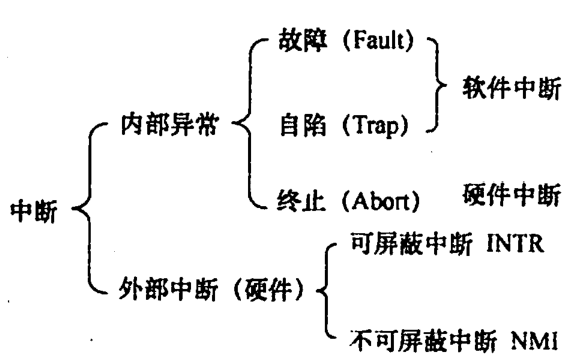
\includegraphics[width=0.6\textwidth]{./images/interrupt.png}
  \caption{异常和中断的联系与区别}
\end{figure}

\begin{itemize}
  \item 异常中的Fault和Trap属于\textbf{软件中断}。
  \item 异常中的Abort和外中断属于\textbf{硬件中断}。
\end{itemize}

中断和异常的区别:
\begin{itemize}
  \item 异常一般是由特定指令在执行过程中产生的,而中断和指令没有关系,也不阻止指令的完成。
  \item 异常的检测由CPU自身完成,不依赖外部信号;中断则是从请求线传进来的信号。
\end{itemize}

\subsubsection{异常和中断响应过程}

可分为几步:关中断、保存断点和程序状态、识别异常和中断并转到相应的处理程序。

\begin{enumerate}
  \item 关中断:指的是禁止相应新的中断。通常是将中断允许(IF)触发器置0。若置1表示开中断。
  \item 保存断点和程序状态:通常保存在栈中,以支持异常/中断的嵌套。程序状态字寄存器PSWR也需要保存。
  \item 识别异常和中断并转到相应的处理程序:注意区分软件识别方式和硬件识别方式,见下。
\end{enumerate}

软件识别和硬件识别:
\begin{itemize}
  \item 软件识别:CPU设置一个异常状态寄存器,记录异常的原因。OS使用统一的查询程序,按照优先级顺序查询该寄存器,先查到的先处理。
  \item 硬件识别:又叫向量中断。异常/中断处理程序的首地址叫\textbf{中断向量},所有中断向量都存在\textbf{中断向量表}中
\end{itemize}
异常主要用软件识别,中断处理两种都用。

\subsection{指令流水线}

\subsubsection{指令流水线的基本概念}

处理机并行性:
\begin{itemize}
  \item 时间并行:将一个任务分解为若干个子任务,每个子任务在不同的部件上并行执行,即流水线技术。
  \item 空间并行:在一个处理机内设置多个执行相同任务的功能部件,令其并行工作,即超标量处理器技术。
\end{itemize}

流水线技术不能缩短单条指令的执行时间,但整个程序的执行效率能够大幅提高。

\subsubsection{流水线的基本实现}

貌似没什么新东西,硬件系统综合设计已经覆盖了全部内容

\subsubsection{流水线的冒险与处理}

赢!体系结构覆盖了本节全部内容

\begin{itemize}
  \item 结构冒险
  \item 数据冒险
  \begin{itemize}
    \item RAW相关
    \item WAR相关
    \item WAW相关
  \end{itemize}
  \item 控制冒险
\end{itemize}

解决数据冒险的方式:流水线暂停、数据前推、编译时指令重排

\subsubsection{流水线的性能指标}

\begin{enumerate}
  \item 吞吐率
  
  指单位时间内流水线完成的任务数量。

  公式没看太懂,用时再补
  \item 加速比
  
  \begin{equation*}
    S_p=\frac{m}{1+(m-1)/n}
  \end{equation*}
  其中,$m$是流水线段数,$n$是执行指令的条数。
  \item 效率
  
  \begin{equation*}
    E=\frac{n}{m+n-1}=\frac{S_p}{m}
  \end{equation*}
  $m$、$n$含义同上。
\end{enumerate}

\subsubsection{高级流水线技术}

\begin{itemize}
  \item 超标量流水线技术:又称动态多发射技术。每个时钟周期可并发多条指令。需要配置多个功能部件。多数超标量CPU都会使用乱序执行。
  \item 超长指令字技术:又称静态多发射技术,由编译程序挖掘并发性,将多条指令组成一条超长的指令。同样需要配置多个功能部件。
  \item 超流水线技术
\end{itemize}

\subsection{多处理器的基本概念}

应该是考纲新增考点,2022考过一题。

这节基本上照抄的《体系结构 量化研究方法》。还需要再看。

\subsubsection{SISD、SIMD、MIMD}

\begin{itemize}
  \item SISD 单指令单数据流
  \item SIMD 单指令多数据流
  \item MISD 多指令单数据流(实际上不存在)
  \item MIMD 多指令多数据流
\end{itemize}

\subsubsection{硬件多线程的基本概念}

\begin{itemize}
  \item 细粒度多线程:多个线程轮流执行指令,线程执行的指令是不相关的,可以乱序并行执行。
  \item 粗粒度多线程:仅当一个程序需要停顿较长时间时(如cache miss),才切换线程。线程切换的开销比细粒度多线程高。
  \item 同时多线程 SMT:在同一个时钟周期中发射多个不同线程的多条指令执行。
\end{itemize}

现代x86处理器的Hyper-threading技术就是基于SMT的。

\subsubsection{多核处理器的基本概念}

\subsubsection{共享内存多处理器的基本概念}

\section{总线}

\subsection{总线概述}

\subsubsection{总线基本概念}

\begin{itemize}
  \item {\bf 定义}
  \item {\bf 总线设备}
  \begin{itemize}
    \item 主设备:获得总线控制权的设备
    \item 从设备:相应从主设备发来的总线命令的设备
  \end{itemize}
  \item {\bf 总线特性}
  \begin{itemize}
    \item 机械特性
    \item 电气特性
    \item 功能特性
    \item 时间特性
  \end{itemize}
\end{itemize}

\subsubsection{总线的分类}

\begin{itemize}
  \item 片内总线:CPU内部的总线
  \item 系统总线:计算机中各个功能部件(CPU、主存、I/O接口)之间的连线。又分:
  \begin{itemize}
    \item 数据总线:双向
    \item 地址总线:单向
    \item 控制总线
  \end{itemize}
  \item I/O总线:主要用于连接低速I/O设备,如USB、PCI总线。
  \item 通信总线:也叫外部总线。用于在计算机系统之间或计算机和其他设备之间进行通信。
\end{itemize}

\subsubsection{系统总线的结构}

\begin{itemize}
  \item 单总线结构:将所有设备挂在同一组总线上。连接情况见图\ref{single-bus-structure}。
  \begin{itemize}
    \item 优点:结构简单、成本低,容易接入新设备。
    \item 缺点:带宽低,负载重,不能并发传输。
  \end{itemize}
  \item 双总线结构:有两条总线:主存总线和I/O总线。连接情况见图\ref{double-bus-structure}。
  \begin{itemize}
    \item 优点:将低速的I/O设备分离出来,实现了存储器总线和I/O主线的分离。
    \item 缺点:需要增加I/O通道等硬件设备。
  \end{itemize}
  \item 三总线结构:包括主存总线、I/O总线和DMA总线。连接情况见图\ref{triple-bus-structure}。
  \begin{itemize}
    \item 优点:提高了I/O设备的性能,提高了系统吞吐量。
    \item 系统工作效率较低。
  \end{itemize}
\end{itemize}

\begin{figure}
  \centering
  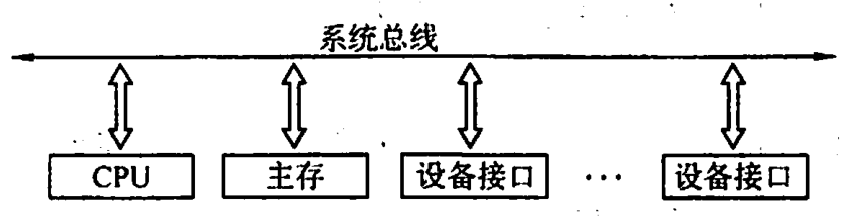
\includegraphics[width=0.6\textwidth]{./images/single-bus-structure.png}
  \caption{单总线结构}
  \label{single-bus-structure}
\end{figure}

\begin{figure}
  \centering
  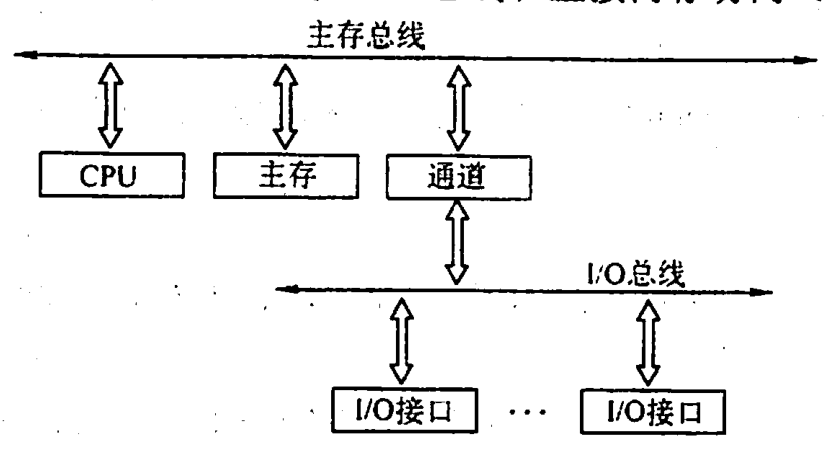
\includegraphics[width=0.6\textwidth]{./images/double-bus-structure.png}
  \caption{双总线结构}
  \label{double-bus-structure}
\end{figure}

\begin{figure}
  \centering
  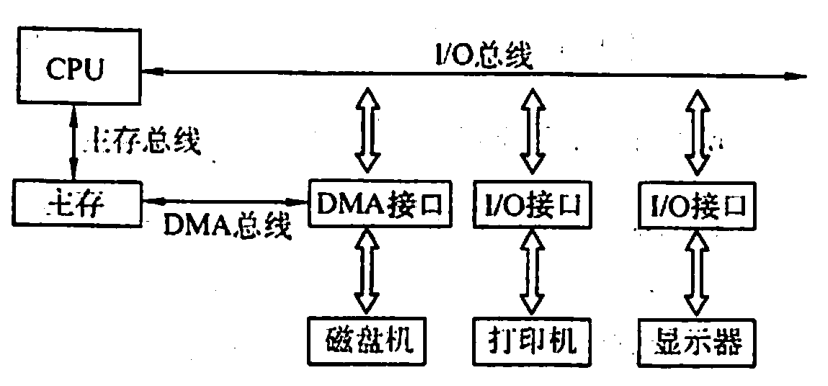
\includegraphics[width=0.6\textwidth]{./images/triple-bus-structure.png}
  \caption{三总线结构}
  \label{triple-bus-structure}
\end{figure}

\subsubsection{常见的总线标准}

很长,有12个之多。只选了其中的一部分内容。详细可见王道2024组成原理P281-282

\begin{enumerate}
  \item ISA,最早的微型计算机系统总线,应用在IBM的AT机上。
  \item EISA,扩展的ISA,完全兼容ISA,为32位系统设计。
  \item VESA,32位局部总线,主要用于多媒体信息如图像的传输。
  \item PCI,32位或64位总线,支持即插即用,和处理器频率无关。
  \item AGP,用于传输视频和三维图形数据。
  \item PCIe,即PCI-Express,全面取代PCI和AGP。
  \item USB,支持即插即用、热插拔。
  \item SATA,由Intel、IBM、Dell提出的硬盘接口规范。
\end{enumerate}

\subsubsection{总线性能指标}

\begin{enumerate}
  \item 总线传输周期,指一次总线操作所需的时间。由若干个总线时钟周期构成。
  \item 总线时钟周期,就是机器的时钟周期。
  \item 总线工作频率,是总线传输周期的倒数。
  \item 总线时钟频率,是总线时钟周期的倒数。
  \item 总线宽度
  \item 总线带宽,=总线工作频率$\times$(总线宽度/8)
  \item 总线复用
  \item 信号线数,指地址总线、数据总线和控制总线加在一起的线路数量。
\end{enumerate}

\subsection{总线事务和定时}

\subsubsection{总线事务}

\begin{enumerate}
  \item 请求阶段。主设备发出传输请求,并获得总线控制权。
  \item 仲裁阶段。总线仲裁机构决定下一个传输周期交给谁。
  \item 寻址阶段。主设备通过总线指定从设备,启动从模块。
  \item 传输阶段。进行数据交换,可单向或双向。一般一次只能传输一个字长的数据。
  \item 释放阶段。主设备让出总线。
\end{enumerate}

猝发(突发)式数据传输允许在传输阶段传输多个连续单元,每个时钟周期仍然只传送一个字长,但可以持续传输而无需反复申请和释放。

\subsubsection{同步定时方式}

使用统一时钟的同步方式。

\begin{itemize}
  \item 优点:速度快,控制简单。
  \item 缺点:不能及时进行数据校验,可靠性差。对于各个部件存取时间相差较大的系统效果不佳。
\end{itemize}

\subsubsection{异步定时方式}

没有同步,完全靠双方握手实现通信。

\begin{itemize}
  \item 优点:灵活,适合各个部件存取时间相差较大的系统。
  \item 缺点:控制稍复杂,速度稍慢。
\end{itemize}

异步方式又可分为:
\begin{itemize}
  \item 不互锁方式。主设备发出请求信号后,无需等待应答,一段时间后自行撤销信号。从设备亦然。
  \item 半互锁方式。主设备需要等待应答,从设备不需要。
  \item 全互锁方式。都需要。
\end{itemize}

\subsection{本章小结}

\begin{problem}
  引入总线结构的好处是?
\end{problem}

\begin{solution}
  \begin{enumerate}
    \item 简化了系统结构,便于设计和制造。
    \item 大大减少了连线数目,便于布线和减小体积。系统可靠性高。
    \item 便于接口设计。
    \item 便于系统的扩充。
    \item 便于设备的软件设计。
    \item 便于故障的诊断和维修。
  \end{enumerate}
\end{solution}

\section{输入/输出系统}

\subsection{I/O系统基本概念}

本节已从新大纲中删除。此处仅选择少部分内容记录。

\subsubsection{I/O系统}

\subsubsection{I/O控制方式}

\begin{itemize}
  \item 程序查询方式
  \item 程序中断方式
  \item DMA方式
  \item 通道方式
\end{itemize}

前两者适合低速设备,后两者适合高速设备。

\subsubsection{外部设备}

\subsection{I/O接口}

\subsubsection{I/O接口的功能}

\begin{itemize}
  \item 进行地址译码和设备选择
  \item 实现主机和外设的通信联络控制
  \item 实现数据缓冲
  \item 信号格式的转换
  \item 传送控制命令和状态信息
\end{itemize}

\subsubsection{I/O接口的类型}

\begin{itemize}
  \item 根据(接口和外设之间的)数据传输方式可分为:
  \begin{itemize}
    \item 并行接口
    \item 串行接口
  \end{itemize}
  \item 按主机的控制方式可分为:
  \begin{itemize}
    \item 程序查询接口
    \item 中断接口
    \item DMA接口
  \end{itemize}
  \item 按功能选择的灵活性可分为:
  \begin{itemize}
    \item 可编程接口
    \item 不可编程接口
  \end{itemize}
\end{itemize}

\subsubsection{I/O端口及其编址}

I/O端口的编址方式:
\begin{itemize}
  \item {\kaishu 统一编址},又叫存储器映射方式。把I/O端口当作存储器的单元进行地址分配。无需设置I/O指令,直接通过访存指令即可访问I/O端口。
  \item {\kaishu 独立编址},又叫I/O映射方式。需要设置I/O指令。
\end{itemize}

\subsection{I/O方式}

这节王道书写的稀烂,可以看唐朔飞课本。

\subsubsection{程序查询方式}

CPU和I/O设备串行工作,效率很低。

\subsubsection{程序中断方式}

有一种中断屏蔽字的应用题,待补。

\subsubsection{DMA方式}

\subsection{本章小结}

\begin{problem}
  CPU响应中断应具备哪些条件?
\end{problem}

\begin{solution}
  \begin{enumerate}
    \item 在CPU内部设置的中断屏蔽触发器是开放的。
    \item 外设有中断请求时,中断请求触发器必须是”1“状态。
    \item 外设(接口)的中断允许触发器是”1“状态。
  \end{enumerate}
  具备上述三个条件时,CPU在现行指令结束的最后一个状态周期响应中断。
\end{solution}

\end{document}